Shellshock, which is also known as Bashdoor, is a vulnerability in the Unix Bash shell. The shell is widely used on servers for internal communication and a range of other functionality. This report will investigate a apache web server utilizing a CGI\cite{CGI} shell script to render some content. Other vulnerable interface are OpenSSH, DHCP clients and Qmail servers\cite{opsxcq}. In the national vulnerability database the exploit has a score of 9.8, which means it is critical\cite{CVE-2014-6271}.  

\subsection*{Vulnerability}
The exploit is enabled by an issue in Bash. In bash you can define an empty function with the following command: 

\begin{lstlisting}
() { :;};
\end{lstlisting}  

Then the problem is that everything you add after the empty function declaration bash sees as executable code. This makes it possible run any arbitrary command after the function declaration. A simple example would be: 

\begin{lstlisting}
() { :;}; echo hello world
\end{lstlisting} 

This will echo hello world. This in itself is not interesting or can not be exploited. But if an attacker was somehow able to make the server call an empty function  body concatenated with a concatenated script, he would have full control of the execution. An example of the error can be seen on figure \ref{fig:vulnerability-echo-vulnerable}

\begin{figure} [ht]
    \centering
    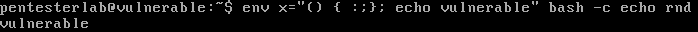
\includegraphics[width=\columnwidth]{../pictures/vulnerability-echo-vulnerable.png}
    \caption{Vulnerability example}
    \label{fig:vulnerability-echo-vulnerable}
\end{figure}

\subsection*{CGI}
An interface where an attacker has a way into utilizing this exploit is CGI. Web servers utilize CGI programs to perform some task on the server. This could be to generate html content based on some parameters received by the requesting user. CGI programs can be implemented in various ways. As this is a bash vulnerability, it has to be bash-based CGI script. The web server, in this case an apache server, will pass http headers to the CGI script. These will then be environment variables in the script and can be accessed in the CGI script. This is the opening for the attacker. He has full control of the headers he will send to the server. He can then set the contents of a header to the empty function declaration concatenated with whatever he wants to execute. The server will then try to set the CGI variable to the contents of the header. But what will happen is that it will see an empty function declaration and execute everything thereafter.  

\subsection*{Reverse shell}
As the attacker can execute any program on the server. An option is to set up a reverse shell. This is a shell session that is established on a connection from a remote machine, in this case the attacker. If an attacker can establish such a connection. He is able to write shell as if he was on the server. 
